\documentclass{beamer}
\usepackage{amsmath}
\usepackage{amsthm}
\usepackage{amssymb}
\usepackage{cite}
\usepackage{xcolor}
\usepackage{enumitem}
\usepackage{graphicx}
\usepackage{caption}
\usepackage{mathtools}
\usepackage[makeroom]{cancel}
\usepackage{sansmathaccent}
\pdfmapfile{+sansmathaccent.map}


\title{Universality in Network Dynamics}
%\subtitle{Introduction and Tutorial}

\begin{document}
\frame{
	\frametitle{Usual Agent Diagram}
	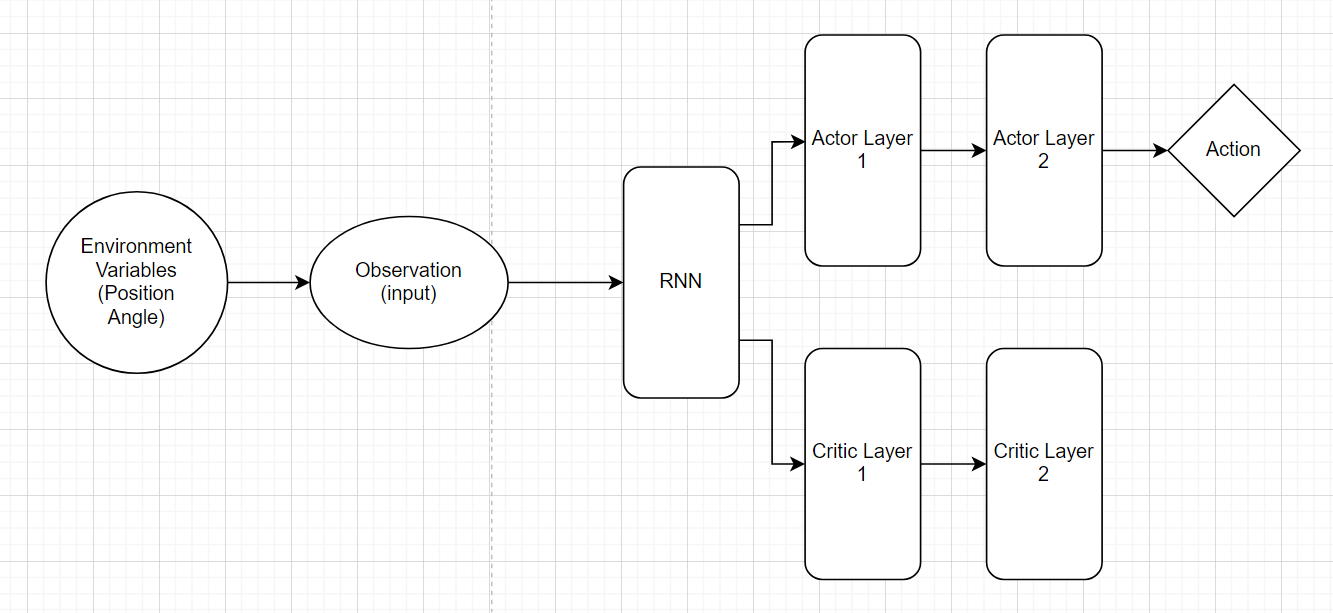
\includegraphics[scale=0.45]{RL diagram1.png}
}
\frame{
	\frametitle{Activations and Position used to train Decoder}
	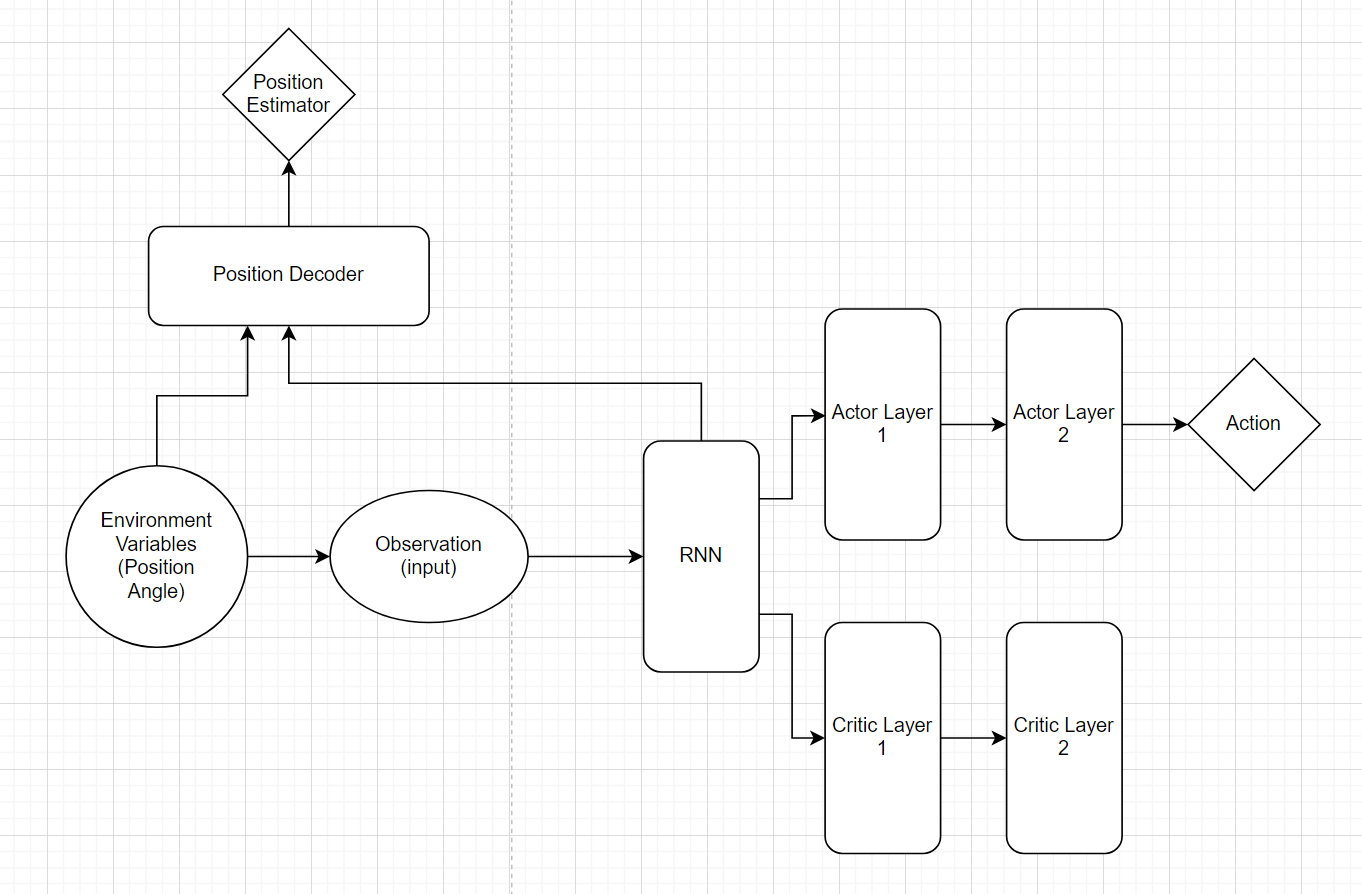
\includegraphics[scale=0.45]{RL diagram2.png}
}
\frame{
	Generate some episodes, record position and activaations of NN during episode
	\begin{figure}
	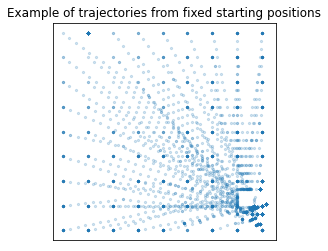
\includegraphics[scale=0.45]{2_1_grid_start_trajectories.png}
	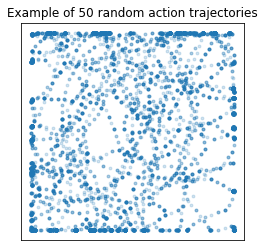
\includegraphics[scale=0.45]{2_2_forced_actions_random_trajectories.png}
	\end{figure}
}
\frame{
	A resulting linear machine learning model can accurately predict position from activations alone (position predicted as which 5x5 grid the agent is currently in)
	\begin{figure}
	\centering
	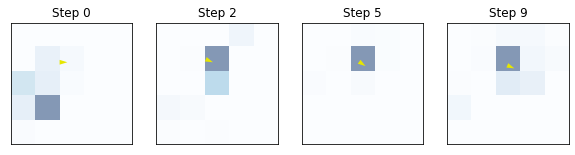
\includegraphics[scale=0.4]{2_2_1_live_episode_decoding.png}
	\end{figure}
}
\frame{
	Position decoders can consistently be trained (Basic 4 wall color task)
	\begin{figure}
	\centering
		\includegraphics[scale=0.3]{4_1_c4_aux_model_classifier_accuracies.png}	
	\end{figure}
	Accuracy seems to drop off for deeper layers
}

\frame{
	\begin{figure}
	\centering
	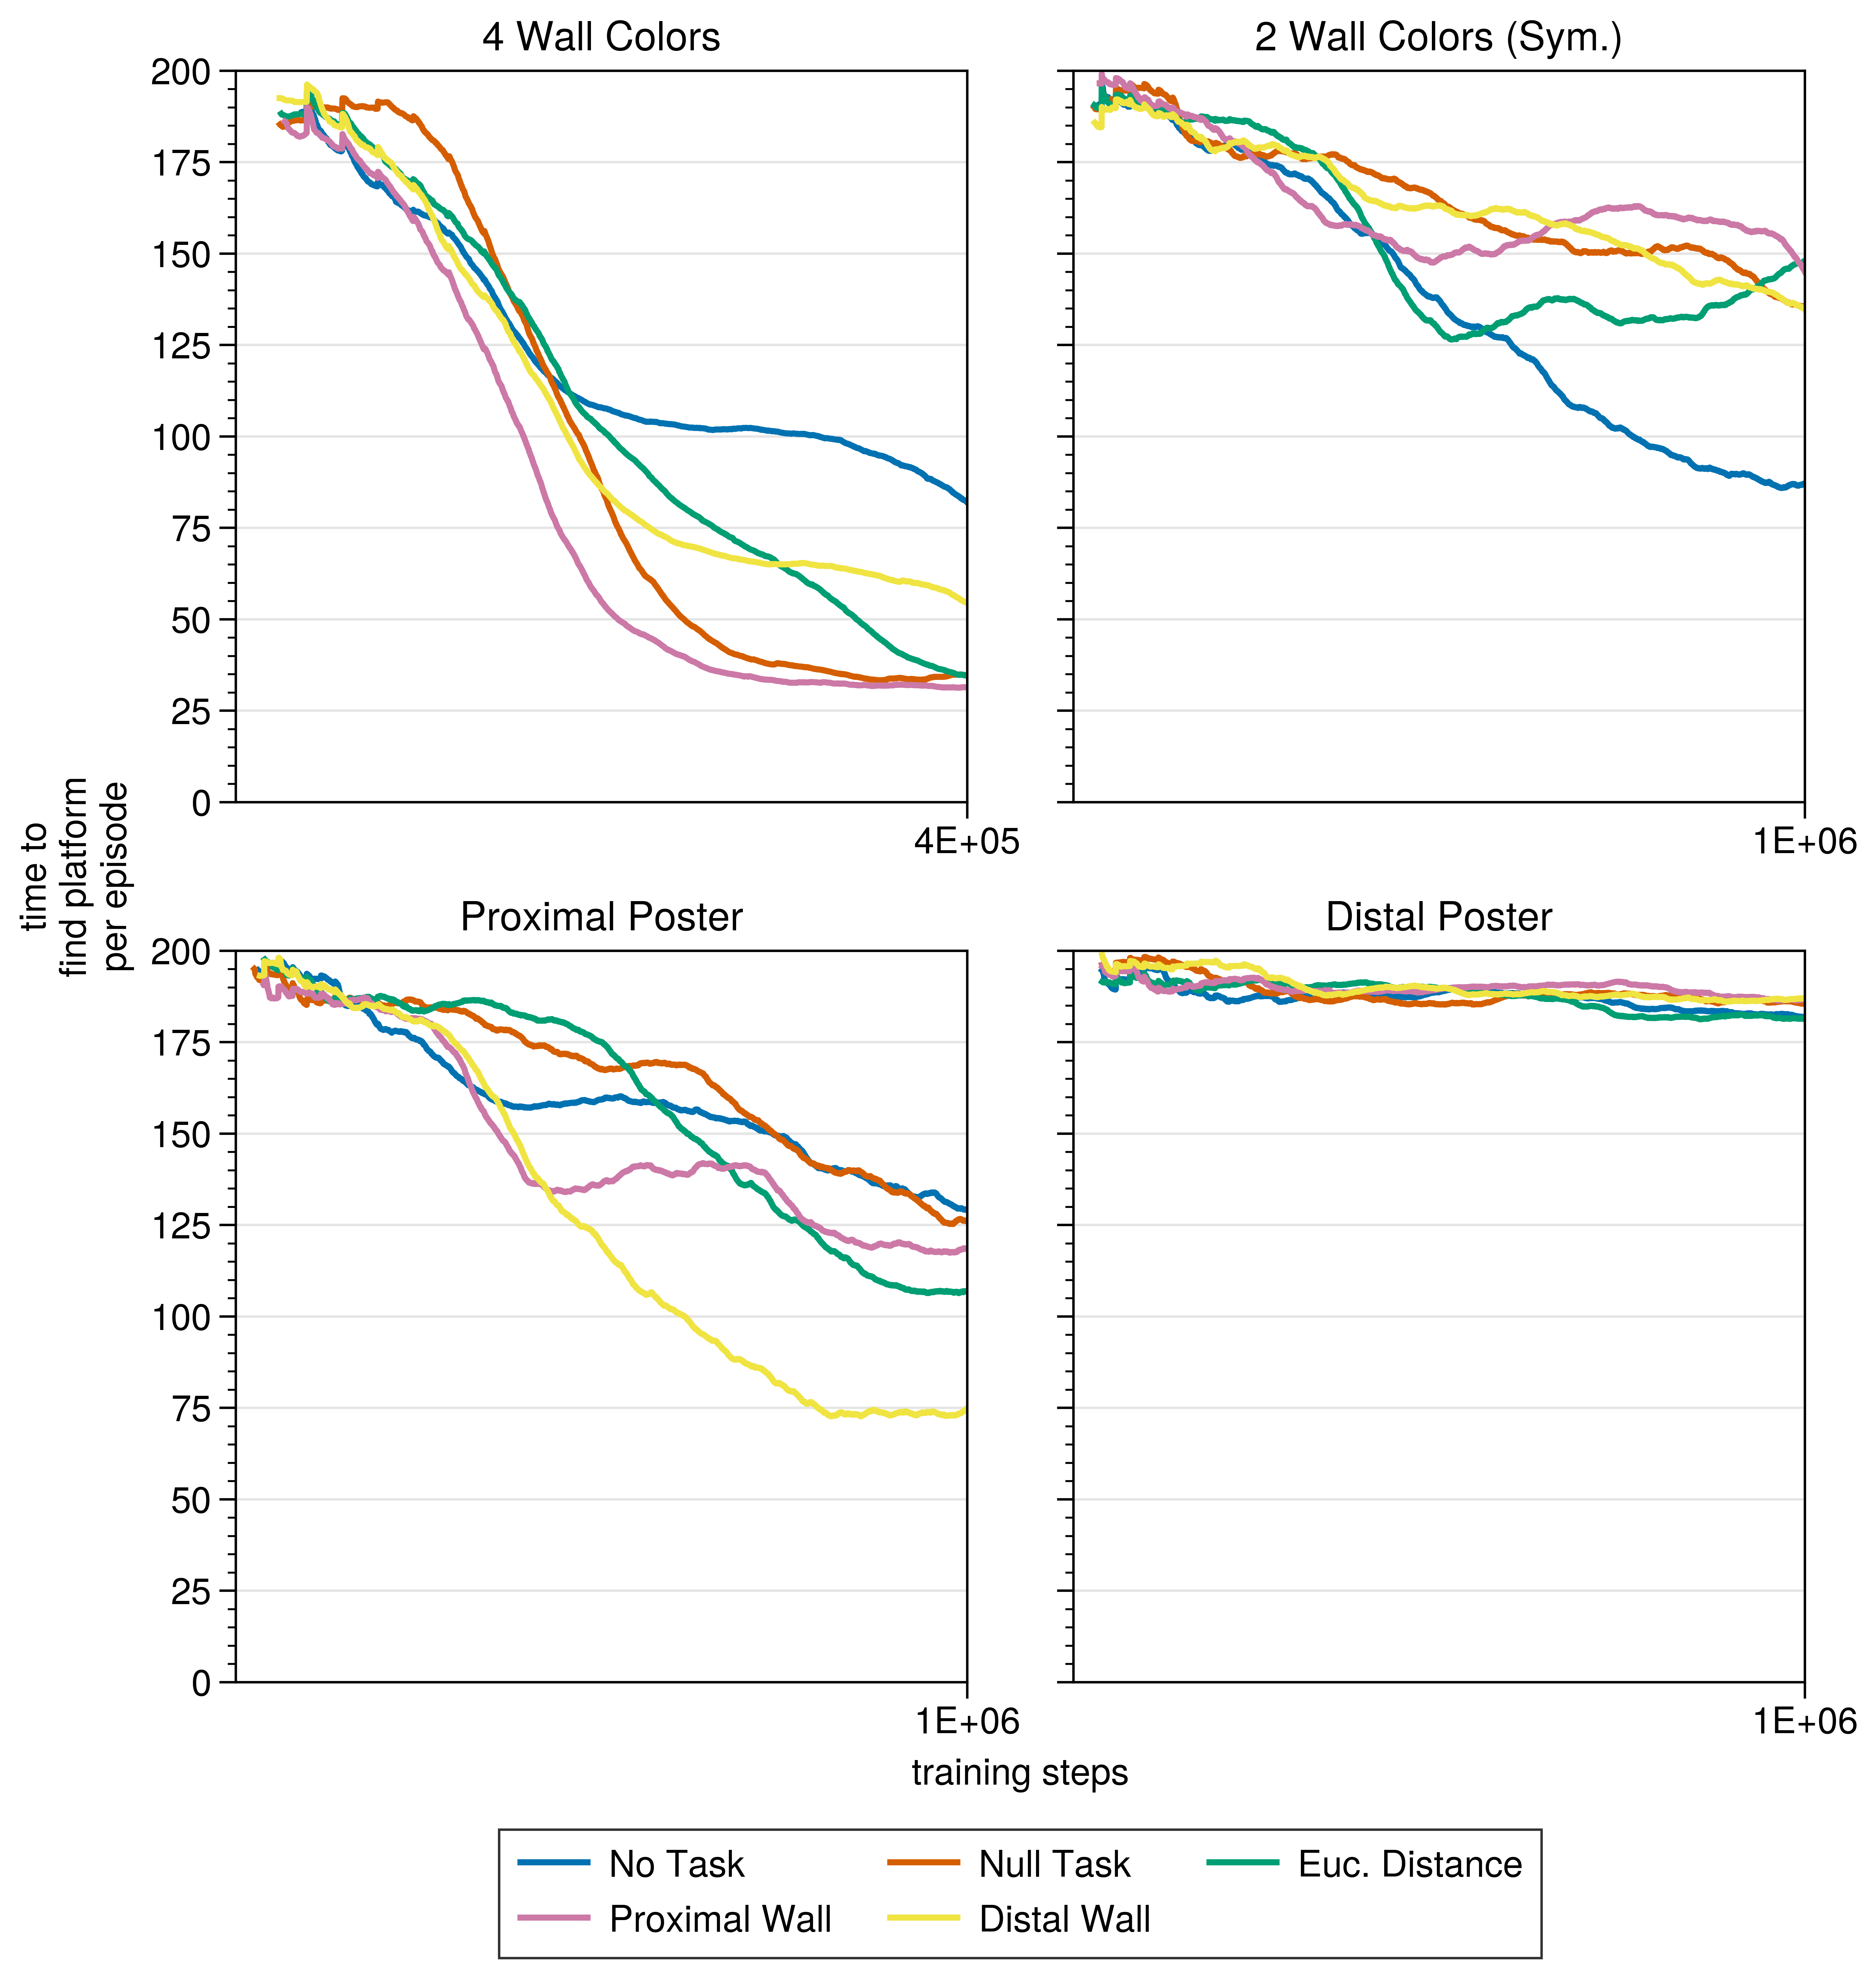
\includegraphics[scale=0.4]{9_1_nav_c4_aux_learning_curves_new.png}
\end{figure}		
}


\frame{
	Position decoders less accurate for proximal poster environment
	\begin{figure}
	\includegraphics[scale=0.3]{4_3_pproxim_aux_model_classifier_accuracies.png}
	\end{figure}
}

\frame{
	Accuracy does not show the whole picture. A position decoder can still achieve about 0.4 accuracy given activations from a totally untrained agent.
	
	\begin{figure}
	\centering
	
\includegraphics[scale=0.4]{5_1_untrainedpolicy_live_episode_decoding.png}
	\end{figure}
}

\frame{
	\frametitle{Questions}
	Does "having good representations" correlate with performance?
	
	Can we quantify what good representations are?
	
	What are deeper layers representing?
}

\frame{
	\frametitle{Exploration of Behavior and Representations}
	
	Proximal Poster environment leads to interesting policy and position decoder
	
	\begin{figure}
	\centering
	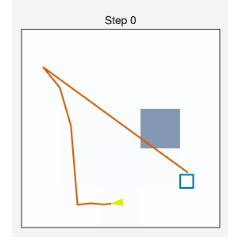
\includegraphics[scale=1]{pproxim trajectory.png}
	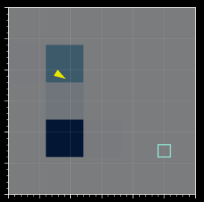
\includegraphics[scale=1]{pproxim sym decode.png}
	\end{figure}
	Left: a sample trajectory of proximal poster environment
	
	Right: a sample step where the position decoder guesses the agent to be in symmetrical position
}

\frame{
	\frametitle{Coloring Neuron Activations}
	(4 Wall Color env) Starting from outer edge, track position and activations for first layer
	
	\begin{figure}
	\centering
	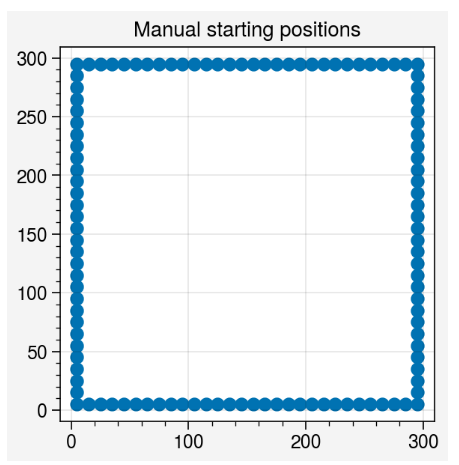
\includegraphics[scale=0.3]{c4_pol_start.png}
	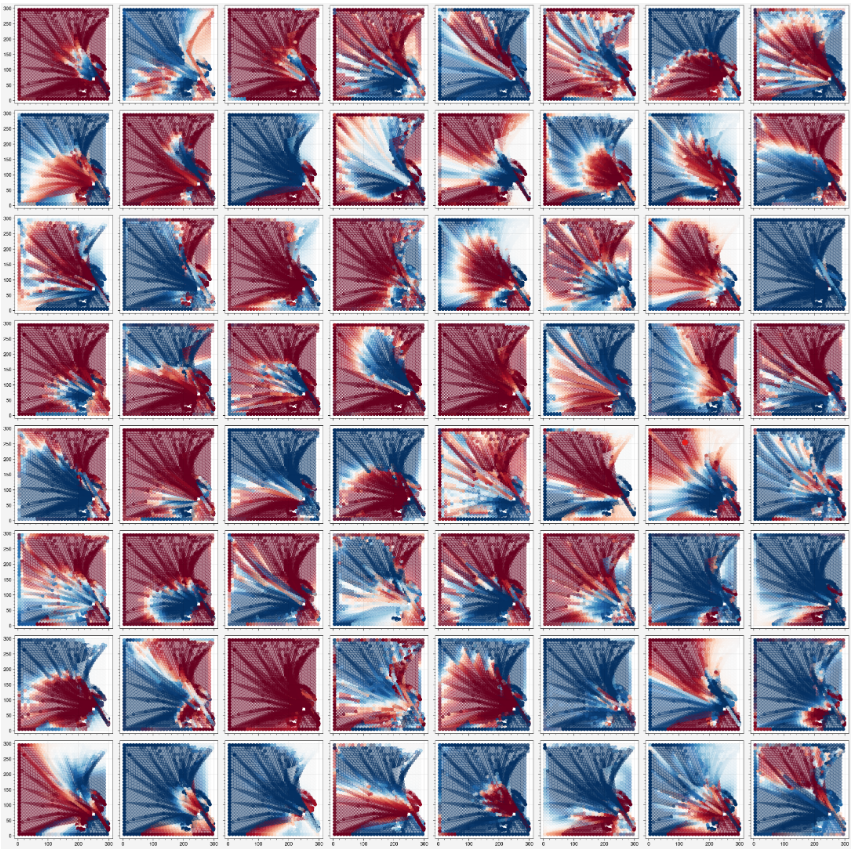
\includegraphics[scale=0.3]{c4_NN_coloringpol.png}
	\end{figure}
}

\frame{
	\frametitle{Coloring Neuron Activations}
	Same env, but fixed actions of moving toward bottom right
	\begin{figure}
	\centering
	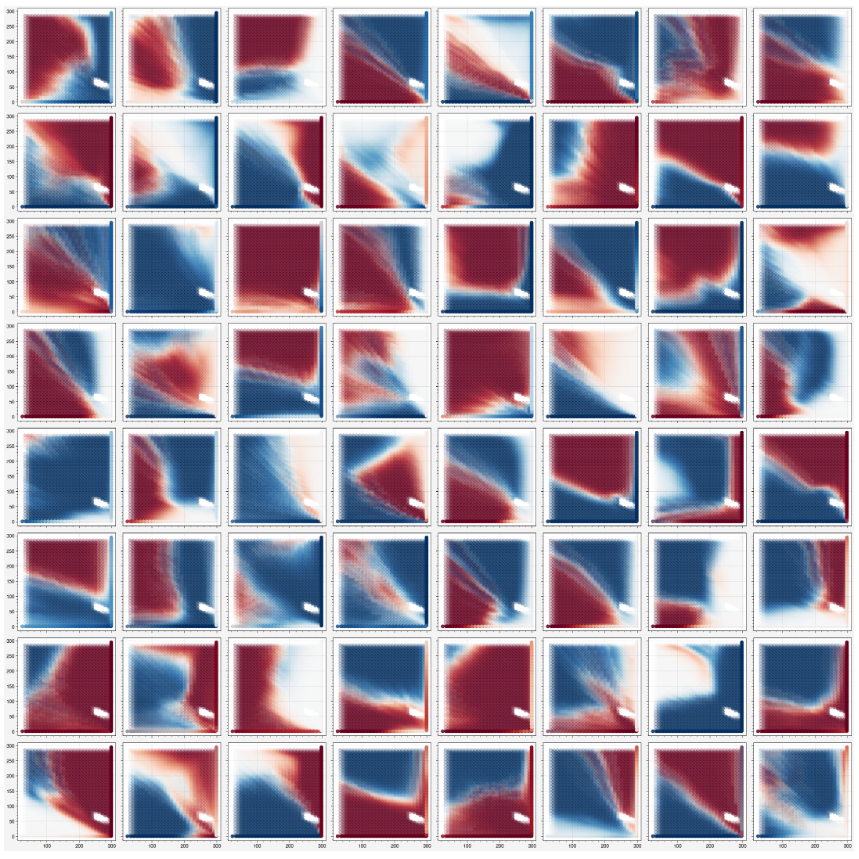
\includegraphics[scale=0.3]{c4_NN_coloring1.png}	
	\end{figure}
}

\frame{
	For comparison
	\begin{figure}
	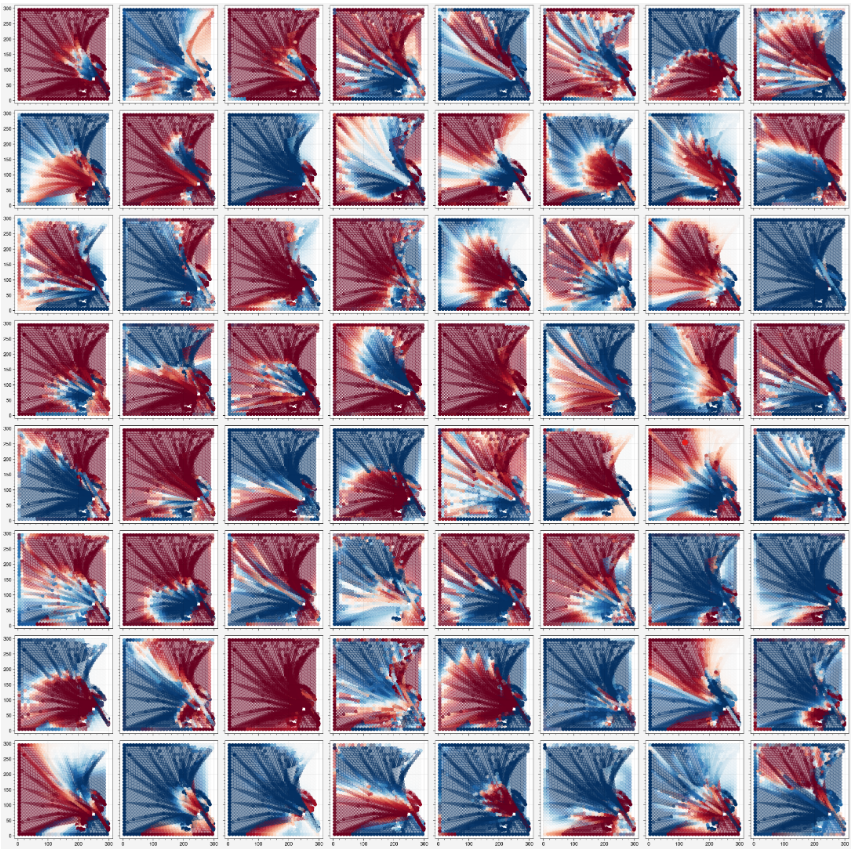
\includegraphics[scale=0.25]{c4_NN_coloringpol.png}
	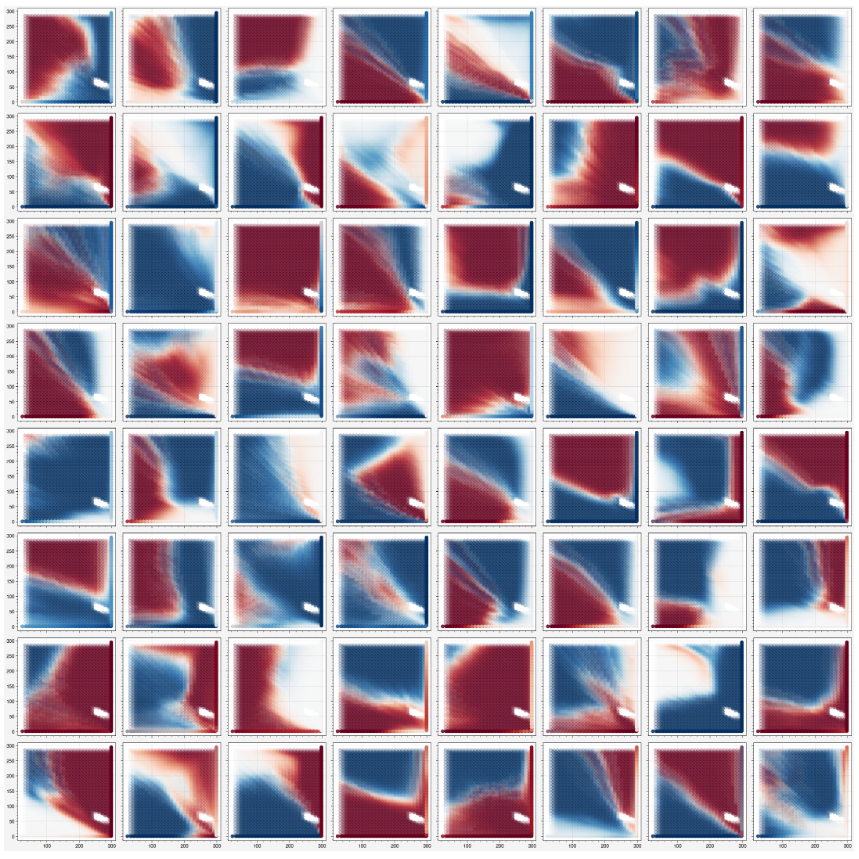
\includegraphics[scale=0.25]{c4_NN_coloring1.png}
	\end{figure}
}

\frame{
	\frametitle{UMAP reducing all activations}
	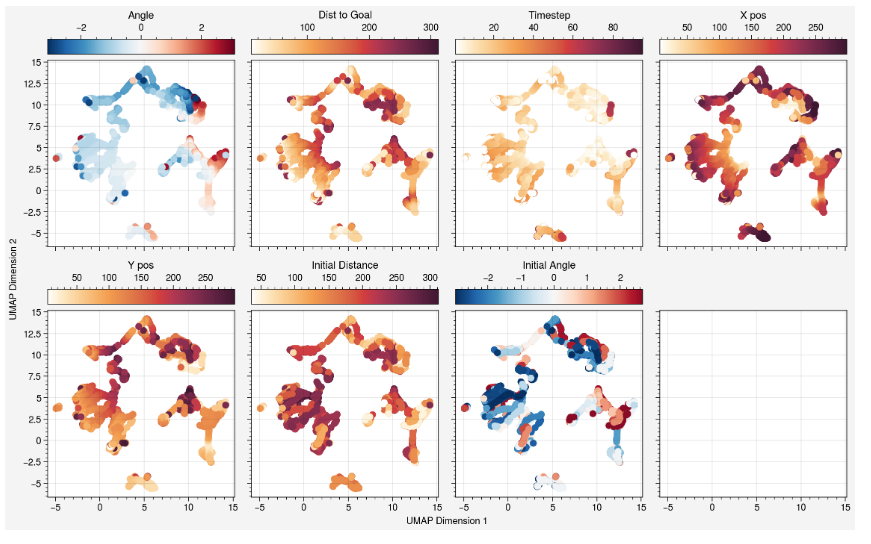
\includegraphics[scale=0.6]{umap_reduce_examples.png}
}
\end{document}